% \documentclass[12pt,a4paper]{article}

% \usepackage[ngerman]{babel}
% \usepackage[T1]{fontenc}
% \usepackage[utf8]{inputenc}
% \usepackage{csquotes}
% \usepackage{amsmath,amssymb}
% \usepackage{geometry}
% \usepackage{setspace}
% \usepackage{hyperref}
% \usepackage{graphicx}
% \usepackage{float}
% \usepackage{tikz}
% \usetikzlibrary{arrows.meta, positioning}




% \geometry{margin=2.5cm}
% \onehalfspacing

% \title{Kapitel 3 -- Methodik und Versuchsdesign}
% \author{}
% \date{}

% \begin{document}
% \maketitle

\section{Methodik und Versuchsdesign}

Um die strukturelle Robustheit eines Smart Grids gegenüber Störungen zu untersuchen, soll analysiert werden, inwiefern die Netzwerkstruktur und die Interdependenzen zwischen Strom- und Kommunikationsnetz die Anfälligkeit des Gesamtsystems gegenüber zufälligen Ausfällen und gezielten Angriffen beeinflussen. Hierfür werden im Folgenden die Modellierung der Netzwerke und das Versuchsdesign dargelegt. 

\subsection{Netzwerkmodelle}
Das Smart Grid wird als System aus zwei gekoppelten Netzwerken modelliert: Einem Stromnetz ud einem Kommunikationsnetz. Beide Netze werden jeweils als Graphen beschrieben, deren Knoten physische bzw.\ informationstechnische Komponenten repräsentieren und deren Kanten physische Leitungen oder Kommunikationsverbindungen abbilden. Diese Abstraktion ermöglicht es, strukturelle Eigenschaften unabhängig von detaillierteren physikalischen Modellen und unabhängig von dynamischen Lastflüssen zu analysieren und somit den Fokus auf die Konnektivität und Fragmentierung zu legen. 

Die Abhängigkeit zwischen Strom- und Kommunikationsnetz werden dabei nicht als vollständige Eins-zu-eins-Verbindung modelliert, wie bei Buldyrev et al. 2010, sondern davon abweichend, als partielle, funktionale Interdependenzen: Für eine realistischere Modellierung repräsentieren einzelne Kommunikationsknoten aggregierte Steuer- und Leitsysteme, von denen mehrere Stromknoten abhängig sind (vgl. Parshani et al. 2010, S. 2; vgl. Yagan et al. 2012, S. 1709). 

Die gewählte Methodik erlaubt es, grundlegende Verwundbarkeiten zu identifizieren, die aus der Topologie der Einzelnetze sowie aus ihrer Interdependenzstruktur resultieren (vgl. Buldyrev et al. 2010, S. 1025). Insbesondere können Unterschiede zwischen zufälligen Ausfällen und gezielten Angriffen auf strukturstarke Knoten, zum Einen auf das Stromnetz selbst und zum Anderen auf das Kommunikationsnetz, analysiert werden. 

\subsection{Störungsszenarien}

Zur Bewertung der Robustheit komplexer Netzwerke ist nicht
nur die zugrunde liegende Topologie entscheidend, sondern auch die Art der
betrachteten Störungen. Unterschiedliche Ausfallmechanismen können sehr
unterschiedliche Auswirkungen auf die Netzwerkstruktur haben. In dieser Arbeit
werden zwei grundlegende Klassen von Störungsszenarien untersucht: zufällige
Ausfälle einzelner Knoten sowie gezielte Angriffe auf strukturell zentrale
Knoten.

\paragraph{Zufällige Ausfälle (Random Failures)}
Zufällige Ausfälle modellieren Störungen, bei denen einzelne Netzkomponenten
ohne systematische Auswahl ausfallen. Typische Ursachen sind technische
Defekte, altersbedingte Ausfälle oder lokal begrenzte externe Einwirkungen. In
der Simulation werden diese Szenarien durch eine zufällige Auswahl von Knoten
realisiert, die schrittweise aus dem Netzwerk entfernt werden.\\
Formal wird der Ausfallgrad durch den Parameter $q \in [0,1]$ beschrieben, der
den Anteil der entfernten Knoten angibt. Für jeden Wert von $q$ wird eine
entsprechende Anzahl von Knoten zufällig ausgewählt und aus dem ursprünglichen
Netzwerk entfernt. Anschließend werden die strukturellen Eigenschaften des
verbleibenden Netzwerks analysiert.\\
Zufällige Ausfälle dienen in der Netzwerktheorie als Referenzszenario zur
Bewertung der allgemeinen Fehlertoleranz. Insbesondere skalenfreie Netzwerke
zeigen in diesem Fall häufig eine hohe Robustheit, da die Wahrscheinlichkeit
gering ist, dass hochgradige Knoten frühzeitig betroffen sind. Die Ergebnisse aus diesen Szenarien bilden daher eine
wichtige Vergleichsbasis für gezielte Angriffsszenarien.

\paragraph{Gezielte Angriffe auf zentrale Knoten}
Gezielte Angriffe modellieren Störungen, bei denen bewusst solche
Netzkomponenten entfernt werden, die für die Konnektivität oder den Fluss im
Netzwerk von besonderer Bedeutung sind. Diese Szenarien sind insbesondere für
kritische Infrastrukturen relevant, da der Ausfall weniger zentraler Knoten
erhebliche strukturelle Schäden verursachen kann.\\
In dieser Arbeit werden zwei Formen gezielter Angriffe betrachtet. Beim
gradbasierten Angriff werden Knoten in absteigender Reihenfolge ihres
Knotengrads entfernt. Der Knotengrad beschreibt die Anzahl direkter Nachbarn
eines Knotens und dient als einfaches Maß für lokale Vernetzung. Knoten mit
hohem Grad fungieren häufig als Hubs, deren Entfernung zu einer schnellen
Fragmentierung des Netzwerks führen kann.\\
Als zweite Angriffsklasse werden Angriffe auf Basis der Betweenness-Zentralität
untersucht. Die Betweenness-Zentralität misst, wie häufig ein
Knoten auf kürzesten Pfaden zwischen anderen Knoten liegt, und erfasst damit
seine Bedeutung für den globalen Informations- oder Leistungsfluss. Knoten mit
hoher Betweenness wirken häufig als Brücken zwischen ansonsten schwach
verbundenen Teilstrukturen. Ihr Ausfall kann daher selbst bei moderatem
Knotengrad zu einer Aufspaltung des Netzwerks führen.

\paragraph{Implementierung der Störungsszenarien}
Die Umsetzung der Störungsszenarien erfolgt modular innerhalb des Projekts.
Die Bestimmung der Reihenfolge, in der Knoten entfernt werden, ist im Modul
\texttt{src/attacks.py} realisiert. Für zufällige Ausfälle wird eine zufällige
Permutation der Knotenliste erzeugt, während für gezielte Angriffe eine
Sortierung nach dem jeweiligen Zentralitätsmaß erfolgt.\\
Die eigentliche Simulation der Knotenentfernung wird im Modul
\texttt{src/simulation.py} durchgeführt. Für jeden betrachteten Wert von $q$
wird die entsprechende Anzahl von Knoten aus dem Netzwerk entfernt, bevor die
definierten Metriken für das verbleibende Netzwerk berechnet werden. Die klare
Trennung zwischen Angriffsauswahl und Simulation erleichtert die
Nachvollziehbarkeit des Versuchsaufbaus und ermöglicht eine einfache
Erweiterung um zusätzliche Angriffsszenarien.

\paragraph{Begründung der Szenarienauswahl}
Die Kombination aus zufälligen Ausfällen und gezielten Angriffen deckt ein
breites Spektrum realistischer Störungsmechanismen ab. Zufällige Ausfälle
erlauben Aussagen über die allgemeine Fehlertoleranz eines Netzwerks, während
gezielte Angriffe Worst-Case-Szenarien abbilden. Der direkte Vergleich beider
Szenarientypen macht strukturelle Schwächen sichtbar und erlaubt es,
Unterschiede zwischen synthetischen Netzwerkmodellen und realen Stromnetzen
systematisch herauszuarbeiten.


\subsection{Bewertungsmetriken}

Zur quantitativen Bewertung der Robustheit und Fehlertoleranz der
untersuchten Netzwerke werden mehrere komplementäre Metriken herangezogen.
Ziel ist es, sowohl den strukturellen Zerfall des Netzwerks als auch dessen
verbleibende Leistungsfähigkeit unter Störungen abzubilden. Die Auswahl der
Metriken orientiert sich an etablierten Ansätzen der Netzwerktheorie und an
deren praktischer Anwendbarkeit im Kontext von Infrastrukturnetzen.

\paragraph{Größte verbundene Komponente (GCC)}
Eine zentrale Kenngröße zur Bewertung der strukturellen Integrität eines
Netzwerks ist die Größe der größten verbundenen Komponente (Greatest Connected
Component, GCC). Sie beschreibt die Anzahl der Knoten, die nach einer Störung
weiterhin miteinander verbunden sind. Zur Vergleichbarkeit zwischen Netzwerken
unterschiedlicher Größe wird die GCC häufig relativ zur ursprünglichen
Knotenzahl betrachtet.

Formal wird die normierte Größe der größten verbundenen Komponente als


\[
S(q) = \frac{|\text{GCC}(q)|}{N}
\]


definiert, wobei $N$ die ursprüngliche Anzahl der Knoten und $q$ der Anteil der
entfernten Knoten ist. Sinkt $S(q)$ stark ab, deutet dies auf eine
Fragmentierung des Netzwerks hin. Diese Metrik ist besonders geeignet, um
strukturelle Zusammenbrüche zu identifizieren und wird in zahlreichen Arbeiten
zur Robustheitsanalyse verwendet.


\paragraph{Robustheitskurven}
Die Robustheitskurve beschreibt den Verlauf der normierten Größe der größten
verbundenen Komponente $S(q)$ in Abhängigkeit vom Anteil der entfernten Knoten
$q$. Sie stellt somit den schrittweisen Strukturverlust eines Netzwerks unter
zunehmender Störung dar.\\
Robustheitskurven erlauben einen direkten Vergleich unterschiedlicher
Netzwerke und Angriffsszenarien. Flach verlaufende Kurven deuten auf eine hohe
Robustheit hin, während ein steiler Abfall auf eine starke Verwundbarkeit
schließen lässt.Beide Fälle sind schematisch in Abbildung~\ref{fig:netzwerkmodelle_vergleich} dargestellt. 
In der vorliegenden Arbeit werden Robustheitskurven für
zufällige Ausfälle sowie für gezielte Angriffe berechnet und
gegenübergestellt.\\
Die Berechnung und Visualisierung der Robustheitskurven erfolgt projektintern
im Modul \texttt{src/analysis.py}, wobei die benötigten Rohdaten aus den
Simulationsergebnissen aggregiert werden.

\paragraph{Fläche unter der Robustheitskurve (AUC)}
Zur Verdichtung der Robustheitskurven auf eine einzelne skalare Kennzahl wird
die Fläche unter der Robustheitskurve (Area Under the Curve, AUC) berechnet.
Sie entspricht dem Integral von $S(q)$ über den betrachteten Bereich von $q$
und kann als globales Robustheitsmaß interpretiert werden.\\
Ein hoher AUC-Wert weist darauf hin, dass ein großer Teil des Netzwerks auch
bei fortschreitender Knotenentfernung erhalten bleibt. Umgekehrt signalisiert
ein niedriger AUC-Wert eine hohe Anfälligkeit gegenüber Störungen. Die AUC
erlaubt somit eine kompakte quantitative Bewertung der Robustheit und eignet
sich insbesondere für den Vergleich unterschiedlicher Netzwerke oder
Angriffsszenarien.

\begin{figure}[htbp]
  \centering
  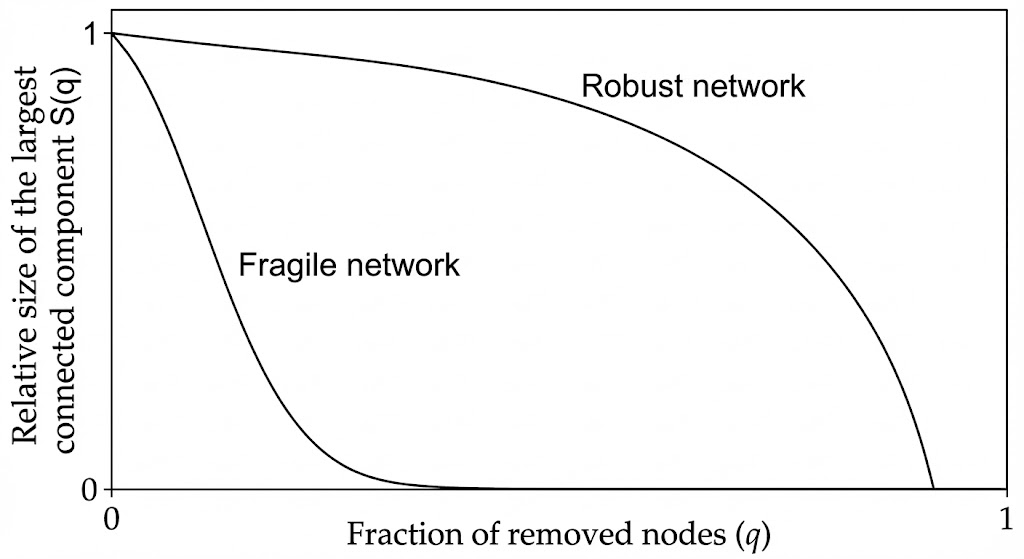
\includegraphics[width=\textwidth]{figures/fragileVsRobustCurves.jpg}
  \caption{Schematische Darstellung von Robustheitskurven für ein robustes
  und ein fragiles Netzwerk.}\label{fig:netzwerkmodelle_vergleich}
\end{figure}

\paragraph{Strukturelle Ergänzungsmetriken}
Neben der Größe der größten verbundenen Komponente werden weitere
strukturelle Metriken betrachtet, um das Robustheitsverhalten genauer
einzuordnen. Dazu zählen insbesondere der Clustering-Koeffizient und der
Durchmesser des Netzwerks.\\
Der Clustering-Koeffizient misst den Grad lokaler Vernetzung und dient als
Indikator für strukturelle Redundanz. Ein hoher Clustering-Wert kann auf
alternative Pfade hinweisen, die zur Fehlertoleranz beitragen. In dieser Arbeit
werden sowohl der globale Clustering-Koeffizient als auch der mittlere lokale
Clustering-Koeffizient berechnet.\\
Der Durchmesser beschreibt die maximale kürzeste Pfadlänge zwischen zwei
Knoten innerhalb der größten verbundenen Komponente. Ein stark ansteigender
Durchmesser im Verlauf der Simulation deutet darauf hin, dass das Netzwerk zwar
noch verbunden ist, jedoch an Effizienz verliert. Der Durchmesser ergänzt damit
die GCC-basierte Analyse um eine Aussage zur erreichbaren Netzwerkleistung.

\paragraph{Implementierung der Metriken}
Die Berechnung der beschriebenen Metriken erfolgt zentral im Modul
\texttt{src/metrics.py}. Dieses Modul kapselt alle Metrikfunktionen und stellt
sicher, dass sie konsistent für synthetische und reale Netzwerke angewendet
werden. Die Aggregation der Ergebnisse sowie die Berechnung der AUC erfolgen in
\texttt{src/analysis.py}. Durch diese Trennung zwischen Simulation und
Auswertung wird eine klare Struktur geschaffen, die sowohl die
Nachvollziehbarkeit als auch die Erweiterbarkeit des Projekts unterstützt.

\subsection{Versuchsprotokoll}

Um die Robustheit unterschiedlicher Netzwerke vergleichbar zu untersuchen,
wird ein einheitliches und reproduzierbares Versuchsprotokoll verwendet.
Dieses legt fest, wie Störungen simuliert werden, in welchen Schritten Knoten
entfernt werden und wie die Ergebnisse aggregiert und gespeichert werden. Ziel
ist es, zufällige Effekte zu kontrollieren und belastbare Aussagen über
strukturelle Unterschiede zwischen den Netzwerken zu ermöglichen.

\paragraph{Anzahl der Wiederholungen}
Da insbesondere zufällige Ausfälle und zufällige Netzgenerierung
stochastischen Schwankungen unterliegen, werden Simulationen mehrfach
wiederholt. Für jedes Netzwerkmodell und jedes Störungsszenario werden mehrere
unabhängige Instanzen erzeugt und ausgewertet. Die Anzahl der Wiederholungen
ist dabei konfigurierbar und wird in den jeweiligen Szenariodateien festgelegt.
Die Wiederholungen dienen dazu, zufällige Ausreißer zu glätten und Mittelwerte
über mehrere Läufe zu bilden. Dies ist insbesondere bei Erdős{-}Rényi- und
Barabási{-}Albert-Netzwerken relevant, da bereits kleine strukturelle
Unterschiede zwischen einzelnen Instanzen das Robustheitsverhalten
beeinflussen können. Die Aggregation über mehrere Läufe erhöht somit die
statistische Aussagekraft der Ergebnisse.

\paragraph{Schrittweite der Knotenentfernung}
Die Entfernung von Knoten erfolgt schrittweise in Abhängigkeit vom
Ausfallparameter $q$, der den Anteil der entfernten Knoten beschreibt. Die
Schrittweite von $q$ bestimmt die Auflösung der Robustheitskurven. Kleine
Schrittweiten ermöglichen eine feinere Analyse des Netzwerkzerfalls, erhöhen
jedoch den Rechenaufwand.\\
In der vorliegenden Arbeit werden typische Schrittweiten zwischen $0{,}02$ und
$0{,}05$ verwendet. Diese stellen einen Kompromiss zwischen Rechenzeit und
analytischer Genauigkeit dar. Die konkreten Werte werden in den jeweiligen
Konfigurationsdateien definiert und können für einzelne Experimente angepasst
werden.

\paragraph{Aggregation der Ergebnisse}
Die Simulationsergebnisse werden für jeden betrachteten Wert von $q$, jedes
Angriffsszenario und jede Netzwerkinstanz separat erfasst. Zur Auswertung
werden diese Rohdaten anschließend aggregiert. Dabei werden für jede
Kombination aus Netzwerktyp und Angriffsszenario Mittelwerte über alle
Wiederholungen gebildet.\\
Die Aggregation erfolgt insbesondere für die Größe der größten verbundenen
Komponente, aus der die Robustheitskurven $S(q)$ abgeleitet werden. Auf Basis
dieser aggregierten Kurven wird anschließend die Fläche unter der Kurve (AUC)
berechnet. Dieses Vorgehen stellt sicher, dass die Robustheitsbewertung nicht
von einzelnen zufälligen Realisierungen dominiert wird.

\paragraph{Reproduzierbarkeit und Zufallsstartwerte}
Ein zentrales Ziel des Versuchsprotokolls ist die vollständige
Reproduzierbarkeit aller Simulationen. Zu diesem Zweck werden alle
zufallsbasierten Prozesse durch explizite Zufallsstartwerte (Seeds) gesteuert.
Dazu zählen sowohl die Generierung synthetischer Netzwerke als auch die
Auswahl zufälliger Ausfallreihenfolgen bei Random-Failure-Szenarien.\\
Die verwendeten Seeds werden in den jeweiligen Konfigurationsdateien
festgelegt. Dadurch kann jede Simulation exakt reproduziert werden, sofern
dieselben Konfigurationsdateien und dieselbe Softwareversion verwendet werden.
Dieses Vorgehen ist insbesondere für den Vergleich von Ergebnissen und für
eine spätere Nachvollziehbarkeit der Experimente von Bedeutung.

\paragraph{Konfigurations- und Ergebnisstruktur}
Alle experimentellen Parameter werden über YAML-basierte
Konfigurationsdateien im Verzeichnis \texttt{configs/} definiert. Diese
enthalten unter anderem Angaben zu Netzwerkmodellen, Angriffsszenarien,
Schrittweiten, Metriken und Wiederholungszahlen. Durch diese Trennung von
Konfiguration und Code können neue Experimente ohne Anpassung der
Implementierung durchgeführt werden.\\
Die Ergebnisse der Simulationen werden strukturiert im Verzeichnis
\texttt{results/} abgelegt. Für jedes Experiment wird ein eigener Unterordner
erzeugt, der sowohl die Rohdaten der Simulationen als auch aggregierte
Auswertungen enthält. Dieses Vorgehen erleichtert die systematische Analyse
der Ergebnisse und bildet die Grundlage für die in Kapitel~5 dargestellten
Resultate.

\newpage
% \nocite{*}
% \bibliographystyle{plain}
% \bibliography{references}

% \end{document}